\subsection{Why the transformer model}\label{sec:transformer intro}
The point of transformers was to overcome the problems faced by the previous state-of-the-art architectures while still including prominent aspects of the RNN and convolutional neural network (CNN) models.

The RNN model has two notable weaknesses. First is its inability to learn long-term patterns due to the exploding and vanishing gradient problems that occur during backpropagation.
Secondly, its recurrent connection is also a weakness. This is because it is not possible to compute the cell at time step $i$ until the cell at time step $i-1$ has been computed as information is propagated along a sequence.
This, in turn, prevents parallelization.

In contrast, one of the benefits of CNNs is that they can be computed concurrently. However, unlike RNNs, they are unable to learn even short-term patterns. The size of the patterns they can learn is limited by their architecture.

Transformers attempt to feature the best of both techniques.
Transformers can model dependencies over the whole range of the input sequence as easily as they can  model neighboring sequences. And there are no recurrent connections, allowing efficient computation using parallelization. This is facilitated through the use of the self-attention mechanism.\cite{TransformersScratchPeterbloem}

\begin{figure}[h]
  \centering
  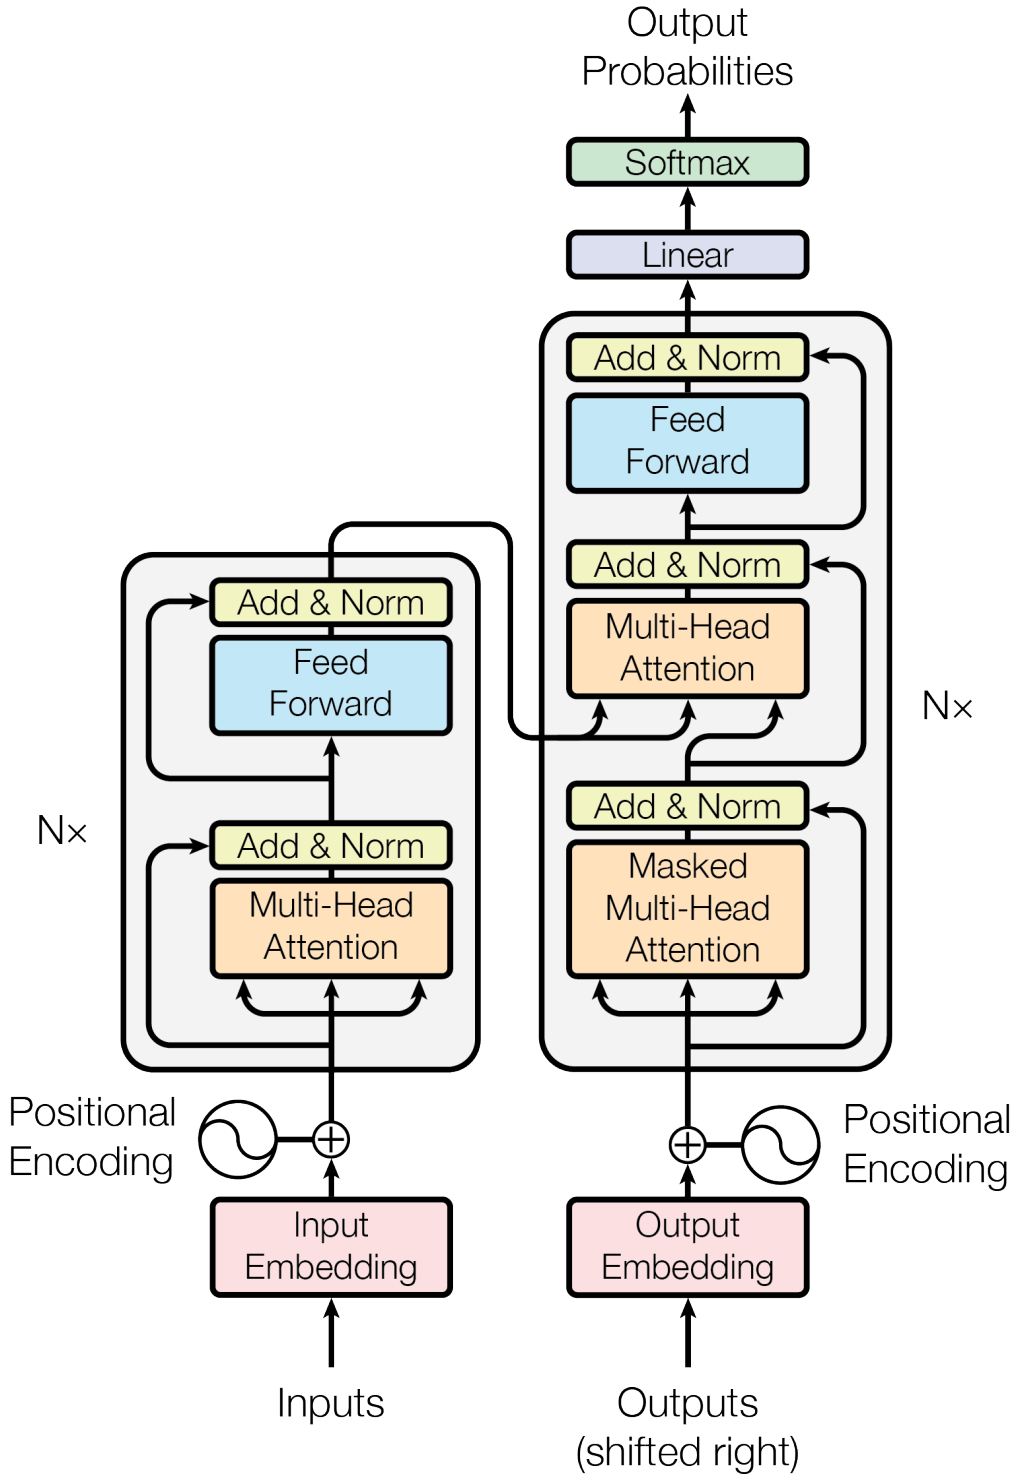
\includegraphics[width=0.5\textwidth]{Transformer model diagram}
  \caption{Diagram depicting the architecture of the transformer model from \citet{AttentionIsAllYouNeed}.}
  \label{fig:original transformer}
\end{figure}